\documentclass{article}

% Geometry for Elsevier Physica B graphical abstract
% Standard requirements: single column width, typically 8.5 cm width
% Height should maintain good aspect ratio, usually ~6-7 cm
\usepackage[
    paperwidth=230mm,
    paperheight=107mm,
    margin=0.0cm,
    noheadfoot
]{geometry}

% Required packages
\usepackage{tikz}
\usepackage{amsmath}
\usepackage{siunitx}
\usepackage{xcolor}
\usepackage{varwidth}

% TikZ libraries
\usetikzlibrary{arrows.meta,shapes.geometric,positioning,decorations.pathreplacing,calc}

% Define colors based on C2DB standards
\definecolor{sbcolor}{RGB}{159,100,181}    % Sb atoms - purple
\definecolor{tecolor}{RGB}{212,122,0}      % Te atoms - orange/gold
\definecolor{bondcolor}{RGB}{100,116,139}  % Bonds - gray
\definecolor{straincolor}{RGB}{220,38,38}  % Strain arrow - red
\definecolor{methodbox}{RGB}{240,248,255}  % Light blue for method box
\definecolor{boxblue}{RGB}{219,234,254}    % Light blue box
\definecolor{boxgreen}{RGB}{220,252,231}   % Light green box
\definecolor{boxyellow}{RGB}{254,243,199}  % Light yellow box
\definecolor{boxpink}{RGB}{252,231,243}    % Light pink box

\pagestyle{empty} % No page numbers or headers

\definecolor{Sb}{RGB}{159, 100, 181}
\definecolor{Te}{RGB}{255, 193, 37}
\tikzset{
    max width/.style args={#1}{
        execute at begin node={\begin{varwidth}{#1}},
        execute at end node={\end{varwidth}}
    }
}

\begin{document}
\begin{tikzpicture}[remember picture, overlay]

\node[anchor=north west,inner sep=0mm](i1) at (current page.north west){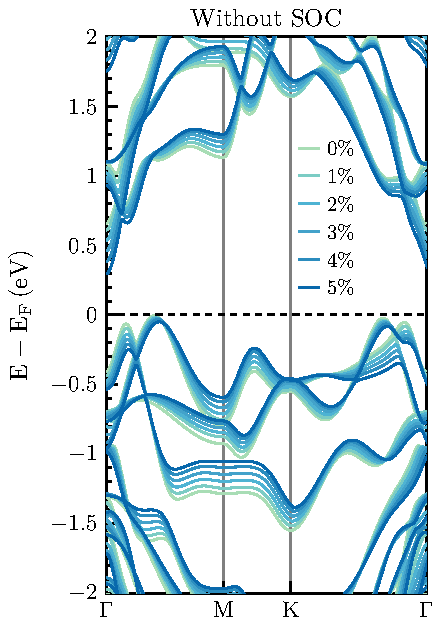
\includegraphics[scale=1]{bands/plot_gga_wou_soc.pdf}};
\node[anchor=north east,inner sep=0mm](i2) at (current page.north east){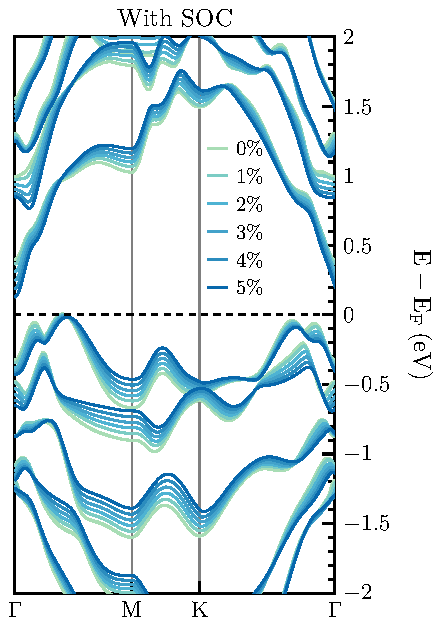
\includegraphics[scale=1]{bands/plot_gga_w_soc.pdf}};
\node[anchor=center](i3) at (current page.center){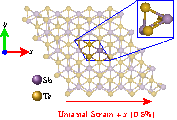
\includegraphics[scale=2.75]{build-oscar/fig_center}};
\node[blue,anchor=north west,shift={(0mm,-1mm)},scale=1.5] at (i1.north west){(a)};
\node[blue,anchor=north east,shift={(0mm,-1mm)},scale=1.5] at (i2.north east){(b)};
\node[blue,anchor=south,shift={(0mm,1mm)},scale=1.5] at (i3.north){(c)};

\end{tikzpicture}

\end{document}